%\documentclass[]{beamer}
\documentclass[handout]{beamer}
%\documentclass[handout,draft]{beamer}
%\documentclass[]{article}


% Preambulo
% Paquetes para usar bien el idioma español
\usepackage[spanish,es-tabla]{babel}
\selectlanguage{spanish}
\usepackage[utf8]{inputenc}

% Paquetes para usar mejores imagenes
\usepackage{graphicx}

% Paquetes para links y tabla de contenidos en el PDF
\usepackage{hyperref}
\hypersetup{colorlinks=true,allcolors=blue}
%\usepackage{hypcap}

% Paquetes para mejores tablas
\usepackage{booktabs}

% Mejor matematica
\usepackage{amsmath}

% Fuentes de las imagenes
\usepackage[absolute,overlay]{textpos}

% Paquete captions
\usepackage[justification=centering,labelformat=empty,labelsep=none]{caption}

% Opciones para ticks
\usepackage{tikz}
\usetikzlibrary{shapes,arrows,positioning}

\tikzstyle{decision} = [diamond, draw, fill=blue!20, text width=4em, text badly centered, node distance=2cm, inner sep=0pt,on grid]
\tikzstyle{block} = [rectangle, draw, fill=blue!20, text width=8em, text centered, rounded corners, minimum height=2em,on grid]
\tikzstyle{line} = [draw, -latex]

% Citas bibliograficas
\usepackage[backend=biber]{biblatex}
\renewcommand{\footnotesize}{\tiny}
\addbibresource{biblio.bib}

% Mejoro las captions
\setbeamertemplate{caption}{\raggedright\insertcaption\par}

\setbeamertemplate{caption}{%
\begin{beamercolorbox}[wd=0.85\paperwidth, sep=.2ex]{block body}\insertcaption%
\end{beamercolorbox}%
}


% Sacar barra de navegacion
\setbeamertemplate{navigation symbols}{}%remove navigation symbols

% Transparencias en items
\setbeamercovered{transparent}

% Estilo de diapositivas
% \usetheme{Boadilla}
\usecolortheme{whale}
\usecolortheme{orchid}

%\usepackage{beamerarticle}

% Titulo
\title{Herramientas de Teledetección Cuantitativa\\{\small Segmentando el espacio mirando para otro lado}}
\author{Francisco Nemiña}

\institute{Unidad de Educación y Formación Masiva \\
Comisión Nacional de Actividades Espaciales}

\logo{
\includegraphics[height=0.7cm]{imagenes/sopi.png}}

\AtBeginSection[]
{
\begin{frame}
\frametitle{Esquema de presentación}
\tableofcontents[currentsection]
\end{frame}
}


\begin{document}
\begin{frame}
    \maketitle
\end{frame}

\section{Escenas del capítulo anterior}
\begin{frame}{La vez pasada vimos}
  \begin{itemize}[<+->]
    \item Que a partir de esto podiamos definir la $\rho_\lambda$ la firma espectral como una característica de cada cuerpo.
    \item Definimos 3 tipos de firmas espectrales \emph{patrón} y como se comportaba cada una.
    \item Que es importante corregir a las imágenes atmosfericamente para obtener el valor de reflectancia del píxel.
    \item Que podemos definir índices a partir de hacer operaciones entre los valores de los píxeles como si fueran números.
    \item Que a partir del concepto de espacio espectral podemos hacer rotaciones que cambian la forma de mostrar la información.
  \end{itemize}
\end{frame}
%--- Next Frame ---%

\section{Clases y categorías}

\begin{frame}{Categorías de uso y cobertura}
  \begin{block}{Definición}
    Hablamos de \emph{categorías de uso y cobertura} cuando hablamos de nuestras categorías de interés para nuestro estudio.
  \end{block}
  \begin{block}{Propiedades}
    Un esquema de clasificación debe ser
    \begin{itemize}[<+.>]
      \item Exaustivo.
      \item Mutuamente excluyente.
      \item Mismo nivel gerarquico.
    \end{itemize}
  \end{block}
\end{frame}
%--- Next Frame ---%

\begin{frame}{Clase espectral}
  \begin{block}{Definición}
    Hablamos de una \emph{clase espectral} cuando hablamos de un conjunto de píxeles que podemos agrupar espectralmente.
  \end{block}
\end{frame}
%--- Next Frame ---%

\begin{frame}{Clave vs. Categoría}
  \begin{block}{Observación}
    Clase espectral y categoría de uso y cobertura \emph{NO} son lo mismo.
  \end{block}
\end{frame}
%--- Next Frame ---%

\begin{frame}{De la imagen...}

    Queremos cambiar de información espectral a categorías. \pause
    \begin{figure}
  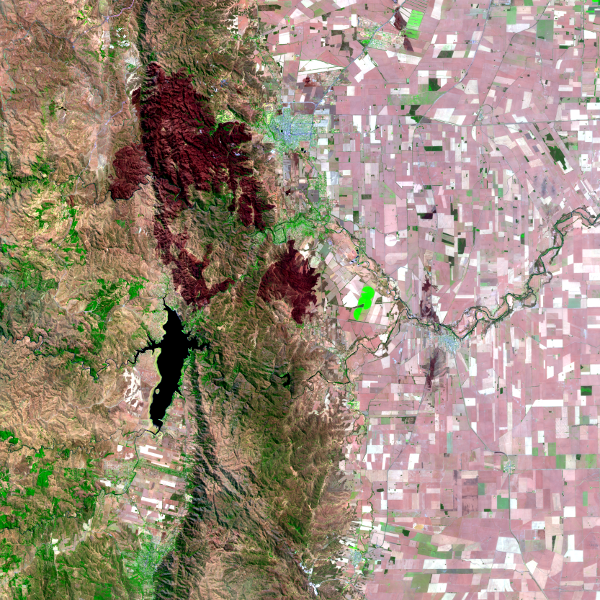
\includegraphics[width=0.6\textwidth]{imagenes/imagen.png}
  \caption{Imagen de la zona de interés en combinación RGB.}
  \end{figure}
\end{frame}
%--- Next Frame ---%

\begin{frame}{...al espacio espectral...}
  \begin{figure}
    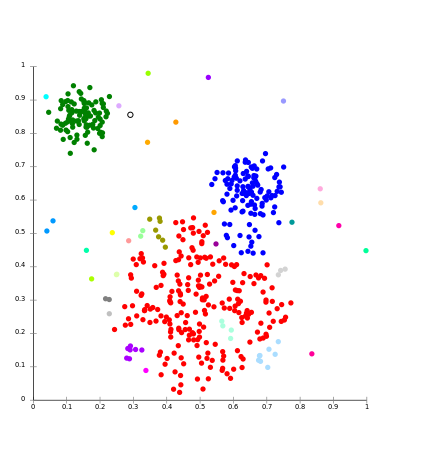
\includegraphics[width=0.5\textwidth]{imagenes/cluster.png}
    \caption{Clustering en $R^2$.\footfullcite{cluster}}
  \end{figure}
\end{frame}
%--- Next Frame ---%

\begin{frame}{... a las categorías}
  \begin{figure}
  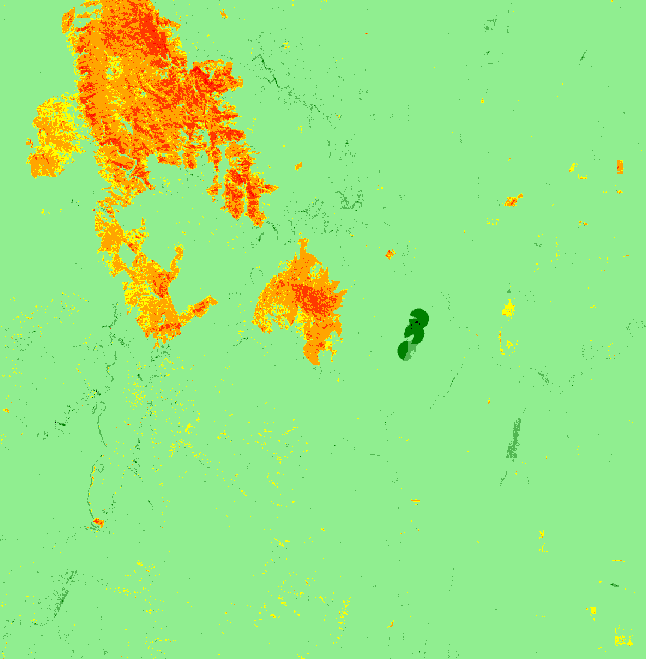
\includegraphics[width=0.6\textwidth]{imagenes/im_class.png}
  \caption{Clasificación de la zona de interés.}
\end{figure}
\end{frame}
%--- Next Frame ---%

\begin{frame}{Objetivo}
  \begin{exampleblock}{¿Cómo?}
    Realizando clasificaciones en el espacio vectorial de la imagen. Estos algoritmos se van a basar en los valores individuales vector píxel.
  \end{exampleblock}
\end{frame}
%--- Next Frame ---%

\section{Clustering}

\subsection{Introducción}

\begin{frame}{Introducción}
  \begin{block}{Distancia}
    Para poder trabajar cómodos en el espacio vectorial vamos a tener que definir la distancia entre dos vectores
    \begin{equation}
    d(\rho_1, \rho_2) = \left( | \rho_{1,i} - \rho_{2,i} |^p \right)^{1/p}
    \end{equation}
  \end{block}
\end{frame}

\begin{frame}{Introducción}
  \begin{exampleblock}{Taxisita}
    Cuando $p=1$ tenemos
    \begin{equation}
      d(\rho_1, \rho_2) = \left( | \rho_{1,i} - \rho_{2,i} | \right)
    \end{equation}
  \end{exampleblock}\pause
  \begin{exampleblock}{Euclídea}
    Cuando $p=2$ tenemos
    \begin{equation}
      d(\rho_1, \rho_2) = \left( | \rho_{1,i} - \rho_{2,i} |^2 \right)^{1/2}
    \end{equation}
  \end{exampleblock}
\end{frame}
%--- Next Frame ---%

\begin{frame}{Introducción}
  \begin{block}{Criterio habitual}
    Encontrar clases $c_i$ que minimice
      \begin{equation}
          SSE = \sum_{c_i} \sum_{x \in c_i} (x-x_i)^2
      \end{equation}
       donde $x_i$ es el promedio de todos los valores de cada clase.
  \end{block}
\end{frame}
%--- Next Frame ---%

\begin{frame}{Introducción}
  \begin{exampleblock}{Una solución}
    Si $c_i = {x_i}$ esto da cero y es mínimo. Entonces tiene al menos una solución.
  \end{exampleblock}\pause
  \begin{block}{Otras soluciones}
    Tenemos que encontrar N categorías $c_i$ que minimicen esto.
  \end{block}
\end{frame}
%--- Next Frame ---%

\begin{frame}{Introducción}
  \begin{block}{Cuentas}
    Esto son MUCHAS cuentas y tomaría mucho tiempo. \pause Tenemos que buscar otra manera más eficiente de hacerlo.
  \end{block}
\end{frame}
%--- Next Frame ---%

\subsection{k-means}
\begin{frame}{k-means}
  \begin{exampleblock}{Ejemplo en 1-D}
    Edades.
  \end{exampleblock}
\end{frame}
%--- Next Frame ---%

\begin{frame}{k-means}
  \begin{figure}
    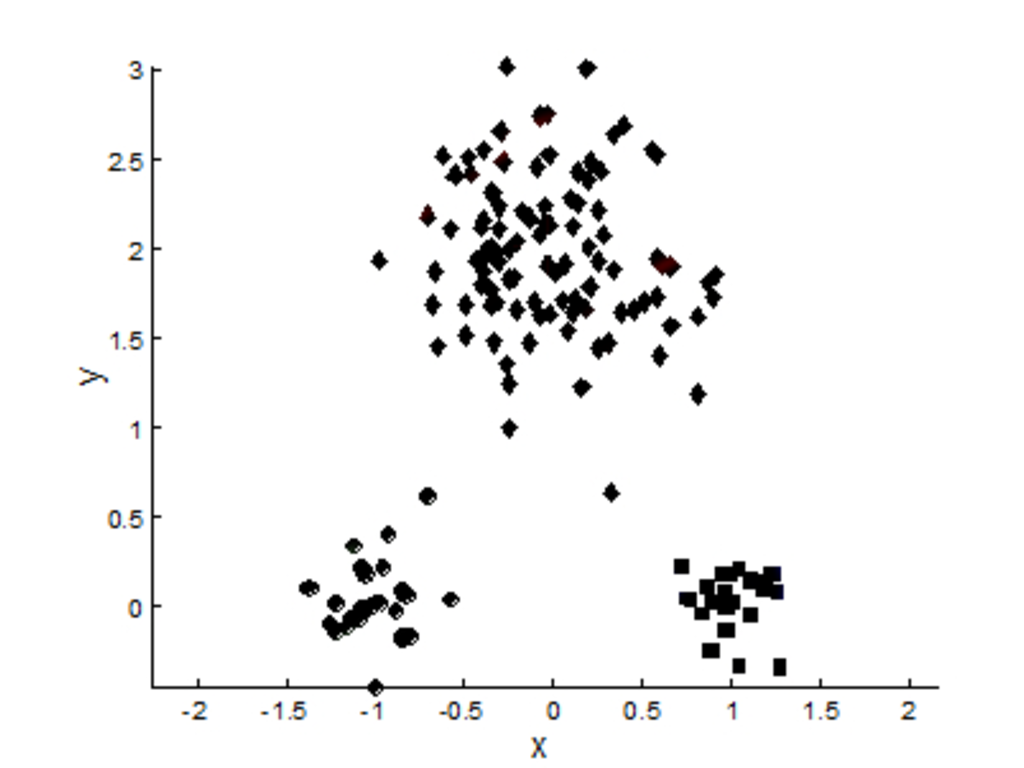
\includegraphics[width=0.6\textwidth]{imagenes/byn.png}
    \caption{Imagen a clasificar.\footfullcite{kmean}}
  \end{figure}
\end{frame}

\begin{frame}{k-means}
  \begin{figure}
    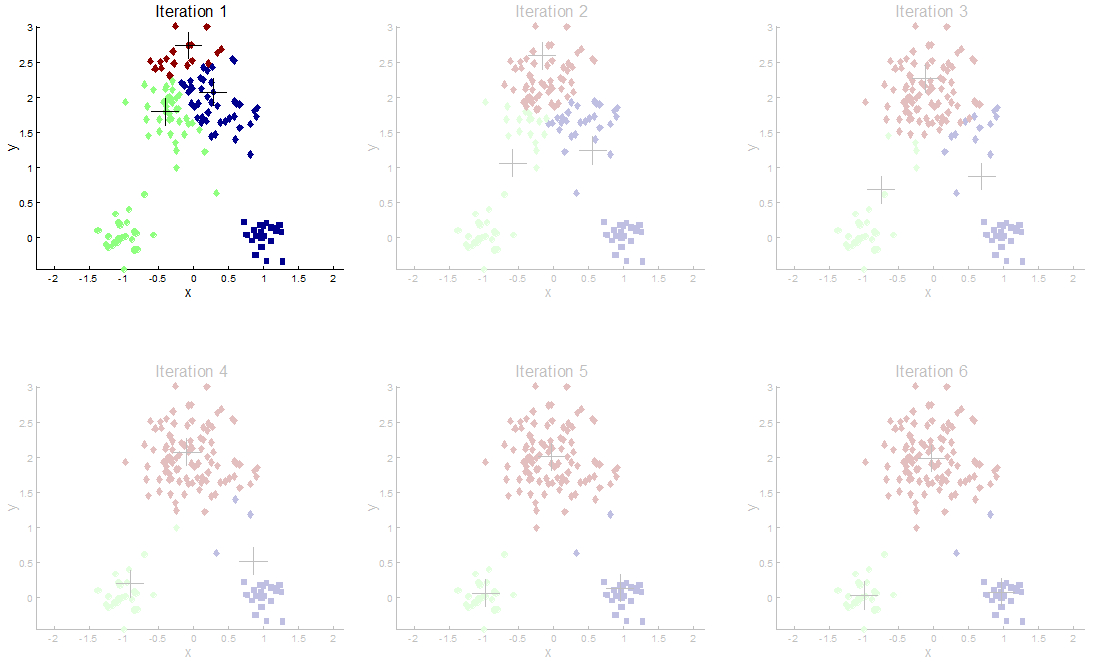
\includegraphics[width=0.9\textwidth]{imagenes/step1.png}
    \caption{Proceso paso a paso.\footfullcite{kmean}}
  \end{figure}
\end{frame}

\begin{frame}{k-means}
  \begin{figure}
    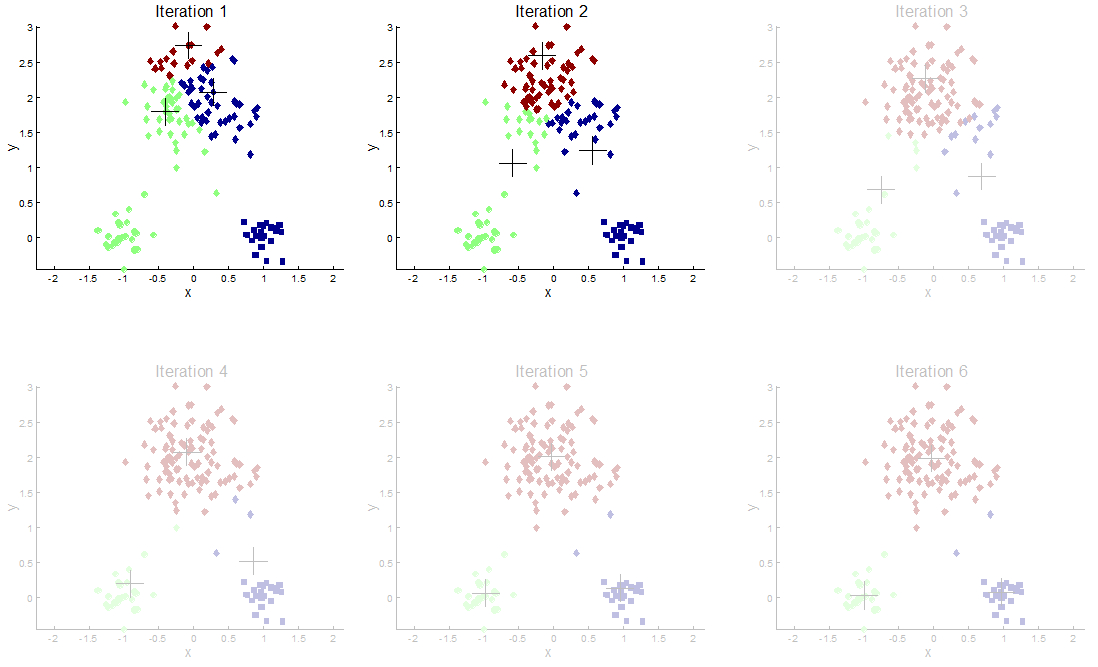
\includegraphics[width=0.9\textwidth]{imagenes/step2.png}
    \caption{Proceso paso a paso.\footfullcite{kmean}}
  \end{figure}
\end{frame}

\begin{frame}{k-means}
  \begin{figure}
    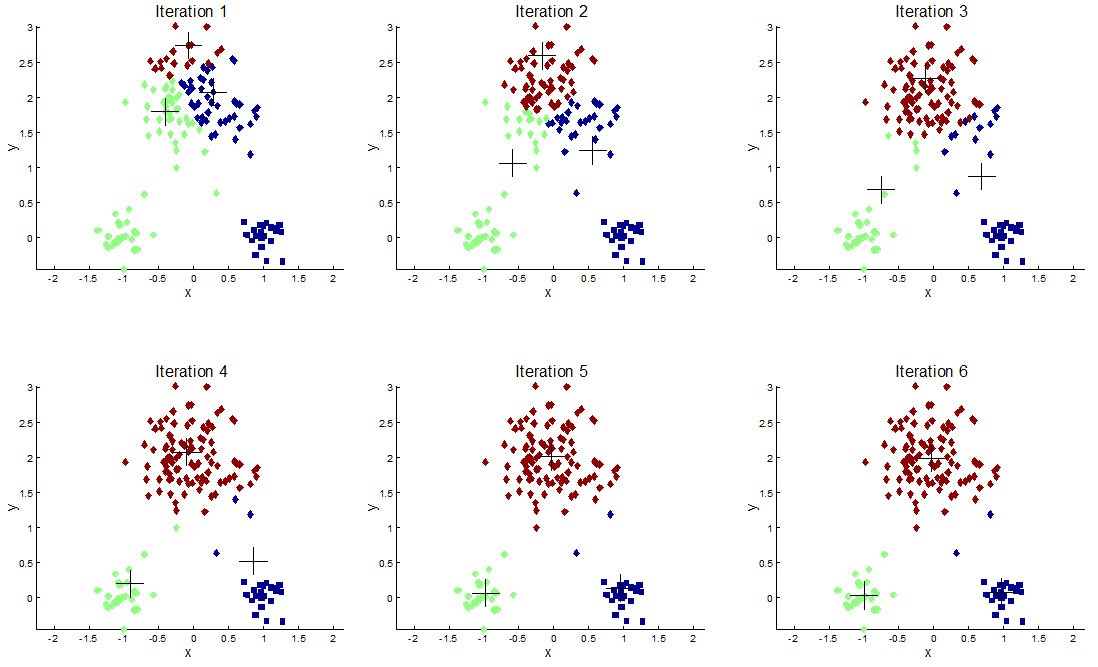
\includegraphics[width=0.9\textwidth]{imagenes/step.png}
    \caption{Proceso paso a paso.\footfullcite{kmean}}
  \end{figure}
\end{frame}

\begin{frame}{k-means}
  \begin{block}{Descripción del algoritmo}
    \begin{enumerate}[<+>]
      \item Selecciono N clases iniciales
      \item Asigno los píxeles a estas clases
      \item Calculo los centroides de las clases clasificadas
      \item Repito 2 - 4 con los nuevos centroides hasta converger
    \end{enumerate}
  \end{block}
\end{frame}
%--- Next Frame ---%

\begin{frame}{k-means}
  \begin{figure}
    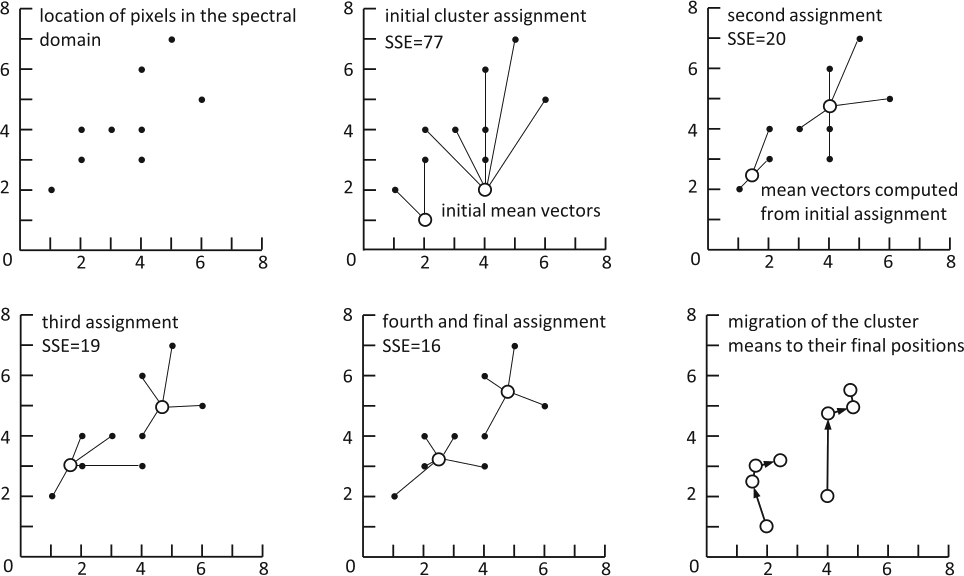
\includegraphics[width=0.8\textwidth]{imagenes/sse.png}
    \caption{Y que pasa con la función de SSE a minimizar. \footfullcite{richards2013remote}}
  \end{figure}
\end{frame}

\subsection{Problemas}

\begin{frame}{Problemas}
  \begin{figure}
    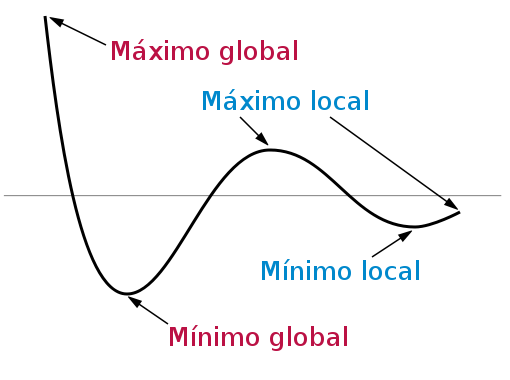
\includegraphics[width=0.8\textwidth]{imagenes/minimo.png}
    \caption{Mínimo local vs. mínimo global en 1-D.\footfullcite{minimo}}
  \end{figure}
\end{frame}
%--- Next Frame ---%

\begin{frame}{Problemas}
  \begin{alertblock}{Selección inicial de clases}
    Lo que determina a que mínimo converge es la selección inicial de clases. Además no siempre me garantizo generar N clases, puedo generar menos de las deseadas.
  \end{alertblock}\pause
  \begin{block}{Como elijo las medias iniciales}
    \begin{itemize}[<+>]
      \item De forma estocástica
      \item Con algún criterio estadístico
    \end{itemize}
  \end{block}
\end{frame}

\subsection{isodata}

\begin{frame}{isodata}
  \begin{block}{Diferencias con respecto a kmeans}
    El algoritmo es básicamente el mismo, pero implementa tres condiciones adicionales.
    \begin{itemize}[<+>]
      \item Eliminar cluster si no son estadísticamente relevantes.
      \item Fusionar cluster si espectralmente son similares.
      \item Partir clusters que son muy alargados.
    \end{itemize}
  \end{block}
\end{frame}

\begin{frame}{isodata}
  \begin{figure}
    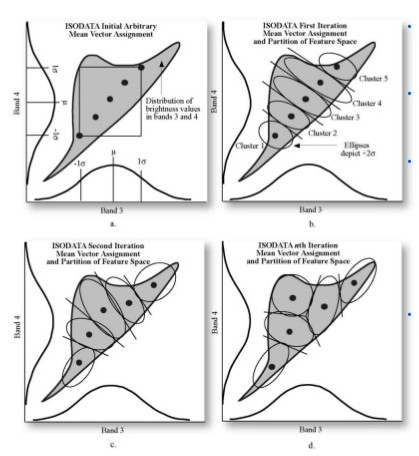
\includegraphics[width=0.6\textwidth]{imagenes/isodata.png}
    \caption{Clasificación no supervisada por isodata.\footfullcite{isodata}}
  \end{figure}
\end{frame}
%--- Next Frame ---%

\section{Práctica}

\begin{frame}{Práctica}
  \begin{exampleblock}{Actividades prácticas de la primera clase}
    \begin{enumerate}
      \item Clasifique la imagen por el método k-means con 7 clases.
      \item Clasifique la imagen por el método k-means con 70 clases.
      \item Utilizar la herramienta de estadísticas globales para estimar las áreas correspondientes a cada uso y cobertura.
    \end{enumerate}
  \end{exampleblock}
\end{frame}
%--- Next Frame ---%

\end{document}
